\section{Related Work}
\label{sec:related_work}

\paragraph{RL for multi-turn LLM agents.}
GRPO~\citep{shao2024deepseekmath}, Proximal Policy Optimization (PPO)~\citep{schulman2017ppo}, and reinforcement learning from human feedback (RLHF) methods~\citep{ouyang2022instructgpt,rafailov2023dpo} have been extended to multi-turn agents~\citep{yao2023react,ragen2025} via step-independent windowing. RAGEN~\citep{ragen2025} introduced this decomposition as a practical solution to memory constraints, partitioning trajectories into fixed-size windows each optimized as independent GRPO samples. Subsequent work builds on this foundation: DigiRL~\citep{digiRL2024} applies online RL to web agents with autonomous reward, SPEAR~\citep{spear2025} addresses entropy collapse through progressive reward scaling, and SelfGuide~\citep{selfguide2026} uses self-generated rewards. These systems inherit the step-independent design without examining its credit assignment implications. Our work identifies this shared choice as a structural failure point.

\paragraph{Credit assignment in RL.}
The credit assignment problem (determining which actions contributed to an outcome) is fundamental to RL~\citep{sutton1988td,williams1992reinforce}. Classical solutions include temporal difference learning, eligibility traces, and generalized advantage estimation~\citep{schulman2016gae} (Appendix~\ref{app:classical_connection}). Step-independent GRPO inherits the worst of outcome-vs-process supervision~\citep{lightman2024lets}: all windows receive episode-level credit regardless of individual action quality. Recent methods address this at different granularities: ArCHer~\citep{zhou2024archer} and VinePPO~\citep{kazemnejad2024vineppo} improve value estimation, PRIME~\citep{prime2025}, VAPO~\citep{vapo2025}, and iStar~\citep{istar2025} refine credit granularity, while GiGPO~\citep{feng2025gigpo}, Turn-PPO~\citep{turnppo2025}, SWEET-RL~\citep{sweetrl2025}, MT-GRPO~\citep{mtgrpo2025}, GAGPO~\citep{gagpo2026}, and HCAPO~\citep{hcapo2026} propose step- or turn-level advantage computation that preserves sign correctness. Our framework provides a unified explanation for \textit{why} these finer-grained methods succeed: they eliminate M2 (sign misattribution) while operating within the windowed framework. IRC~\citep{irc2026}, MC-GRPO~\citep{mcgrpo2026}, GRPO-$\lambda$~\citep{grpolambda2025}, OAR~\citep{oar2026}, and~\citet{gradientcoupling2025} independently corroborate our sign-level diagnosis from complementary perspectives.

\paragraph{GRPO collapse phenomena.}
Training instability under GRPO has been documented across multiple settings. RAGEN-2~\citep{ragen2_2026} and GRPO-Collapse~\citep{grpocollapse2025} report reward variance collapse where all rollouts converge to similar returns, zeroing out advantages. RC-GRPO~\citep{rcgrpo2026} and EDGE-GRPO~\citep{edgegrpo2025} propose variance-preserving modifications. Our dual-mechanism framework subsumes these observations: reward variance collapse is a special case of the reward saturation phenomenon we analyze in Section~\ref{sec:theory}, arising when $\sigma \to 0$ in GRPO normalization. The M1--M2 vicious cycle (where information loss depresses success rate, amplifying sign errors, which further degrade performance) provides a causal mechanism for the empirically observed death spirals.

\begin{figure}[t]
\centering
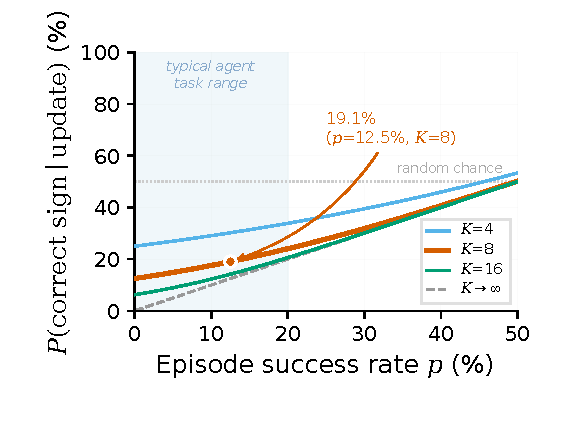
\includegraphics[width=\columnwidth]{fig_theory_curve.pdf}
\caption{Upper bound on the probability of correct gradient sign vs.\ episode success rate $p$ (Proposition~2). At typical agent task success rates ($p < 0.2$, shaded), the majority of gradient updates carry incorrect sign regardless of group size $K$.}
\label{fig:theory_curve}
\end{figure}
